\documentclass[conference]{IEEEtran}
\IEEEoverridecommandlockouts

% ==========================================
% PACKAGES
% ==========================================
\usepackage{cite}
\usepackage{amsmath,amssymb,amsfonts}
\usepackage{algorithmic}
\usepackage{graphicx}
\usepackage{textcomp}
\usepackage{xcolor}
\usepackage{booktabs}
\usepackage{multirow}
\usepackage{url}
\usepackage{float}
\usepackage{hyperref}
\usepackage{listings}

% --- TIKZ (Architectural Diagrams) ---
\usepackage{tikz}
\usetikzlibrary{shapes.geometric, arrows, arrows.meta, positioning, fit, calc, backgrounds, shadows, trees}

% --- CUSTOM STYLING ---
\setlength{\parskip}{0.5em}
\renewcommand{\baselinestretch}{1.0} 

% --- CODE LISTING STYLE ---
\lstset{
    basicstyle=\ttfamily\footnotesize, 
    breaklines=true,
    frame=single,
    numbers=left, 
    numberstyle=\tiny,
    keywordstyle=\color{blue},
    commentstyle=\color{green!60!black},
    stringstyle=\color{red}
}

\def\BibTeX{{\rm B\kern-.05em{\sc i\kern-.025em b}\kern-.08em
    T\kern-.1667em\lower.7ex\hbox{E}\kern-.125emX}}

\begin{document}

\title{A Unified Privacy-First Reference Architecture for Edge-Based Intelligent Campus Systems}

\author{\IEEEauthorblockN{Dr. S. Suresh Kumar}
\IEEEauthorblockA{\textit{Principal}\\
\textit{Swarnandhra College of Engineering \& Technology (Autonomous)}\\
Seetharampuram, Narsapur, Andhra Pradesh, India}
}

\maketitle

\begin{abstract}
Research on intelligent campus systems has often progressed along several largely independent technical trajectories. Hardware designers optimize energy efficiency, machine-learning researchers pursue improved model accuracy, and governance scholars focus on regulatory and ethical frameworks. Because these efforts rarely intersect during early design stages, systems that perform well in controlled laboratory benchmarks can encounter difficulty once exposed to real-world thermal, regulatory, or social constraints.

This study presents a unified reference architecture for privacy-centered edge intelligence designed to reconcile these traditionally separate design concerns. We introduce Constraint-First Architectural Synthesis (CFAS), a design orientation in which strict limitations---such as bounded latency, volatile-only processing, and mandatory governance gating---define the admissible space of computation. The architecture is organized as a vertically layered stack spanning physical substrate constraints, abstraction logic, verification mechanisms, and sociotechnical accountability. 

By tracing the lifecycle of a spatiotemporal event across these layers and formalizing cross-layer execution contracts, we demonstrate how architectural irreversibility and visible privacy mechanisms can be integrated into a coherent deployment model. The resulting framework clarifies how privacy constraints, physical system limits, and institutional governance mechanisms can be integrated into a coherent operational architecture.
\end{abstract}

\begin{IEEEkeywords}
Reference Architecture, System Synthesis, Edge Computing, Privacy-by-Design, Smart Campus, Threat Modeling, Protocol Buffers, Automated Stewardship.
\end{IEEEkeywords}

\section{Introduction}
Deploying intelligent sensing environments within sensitive spaces---such as university campuses, hospitals, or corporate offices---introduces integration challenges extending well beyond algorithmic performance alone. Real-world deployments must reconcile hardware limits, privacy obligations, institutional governance, and human trust simultaneously. Most existing smart-campus systems optimize highly specific attributes in relative isolation. When these independently optimized components are eventually integrated, the resulting architecture often proves unexpectedly brittle in real-world deployments.

For instance, computer vision researchers often optimize models for inference accuracy and bounding-box precision, sometimes overlooking the severe thermal constraints inherent to passively cooled edge devices. Similarly, systems engineers may construct high-throughput video pipelines that maximize network utilization, yet treat user consent and institutional trust as secondary concerns. Meanwhile, privacy researchers frequently propose mathematically pristine cryptographic protocols that impose prohibitive computational overhead on the low-power CPUs required for pervasive edge deployment. 

This fragmentation contributes to what is commonly described as the privacy paradox within intelligent environments. Institutions often desire operational insight, yet stakeholders remain deeply suspicious of opaque surveillance capabilities. Attempting to address this tension with post-hoc policy instruments generally accomplishes little if the underlying technical architecture retains the physical capacity for misuse \cite{b1}.

To address this challenge, we propose an integrated reference architecture that unifies physical limitations, logical reasoning, governance enforcement, and sociotechnical transparency within a single layered model. This cyber-physical ecosystem is engineered to satisfy competing constraints simultaneously: sub-second processing latency, strict privacy mandates (e.g., GDPR/CCPA), harsh hardware endurance limits, and the absolute requirement for social legitimacy \cite{b2}.

This paper is intended to serve as an architectural blueprint. It defines the structural relationships between critical edge subsystems, establishes the mathematical constraints governing the data pipeline, translates theoretical design principles into raw engineering implementations, and explicitly defines the threat model where the system's privacy claims hold operational weight.

\section{Constraint-First Architectural Synthesis}

Conventional feature-driven system design typically begins with functional requirements and subsequently attempts to retrofit security, privacy, and physical constraints. In our experience, this approach frequently produces inefficient workarounds and hidden vulnerabilities when non-negotiable constraints---such as thermal budgets or regulatory mandates---are discovered late in the design cycle.

In contrast, this work adopts Constraint-First Architectural Synthesis (CFAS), a design orientation rooted in safety-critical engineering practice \cite{b15}. Under this model, non-negotiable constraints are identified first (often reflecting physical or regulatory limits), and these constraints strictly dictate the admissible computation classes.

Formally, system functionality is restricted to operations that remain feasible within the defined constraint set. Let $\mathcal{C}$ be the set of strict system constraints (latency limits, memory bounds, privacy mandates) and $\mathcal{F}$ be the set of admissible functionalities. We enforce:
\begin{equation}
    \mathcal{F} \subseteq \text{Feasible}(\mathcal{C})
\end{equation}

Any proposed feature or model must reside entirely within this feasible space. For example, if a highly accurate deep neural network requires processing latency that exceeds the mandated temporal privacy boundary for data destruction, that model is rendered inadmissible by definition. In this framework, accuracy alone cannot override the constraint.

CFAS diverges from generalized \textit{Privacy-by-Design} frameworks by forcing the simultaneous integration of physical thermal limits, sub-second data destruction deadlines, automated governance gating, and sociological visualization requirements into a single cohesive equation. Effectively, it draws a hard operational perimeter around what the edge node is physically permitted to do.

\section{The Threat Landscape and Architectural Defense Mapping}

Architectural privacy guarantees cannot be interpreted meaningfully without an explicit threat model. The formal adversary capability algebra---defining a tiered classification ($A_0$--$A_4$) with explicit observable, modifiable, and privilege domains---is established in companion work on formal threat modeling \cite{b20_threat}. This section maps each adversary tier to the specific architectural stratum that neutralizes its capabilities.

\textbf{$A_0$ (Passive Observer) $\to$ Physics Stratum:} An attacker sniffing ambient wireless signals or monitoring physical device LEDs. 
\textit{Architectural Defense:} Transparent physical signaling (Privacy LED) and mandatory TLS 1.3 transport encryption at the network boundary.

\textbf{$A_1$ (Local User-Space) $\to$ Logic Stratum:} An entity with non-root access to the edge device. 
\textit{Architectural Defense:} Strict process isolation and volatile-only processing. Raw data buffers are architecturally prohibited from residing in any shared memory region accessible to unprivileged processes.

\textbf{$A_2$ (Remote Network) $\to$ Logic Stratum:} An attacker controlling local network routing to force buffer overflows. 
\textit{Architectural Defense:} Fixed-size queue limits coupled with fail-closed Time-to-Live (TTL) enforcement. The system will always prioritize data destruction over guaranteed network transmission.

\textbf{$A_3$ (Root Administrator) $\to$ Verification Stratum:} An insider attempting retrospective mass surveillance via live memory dumps or disk inspection. 
\textit{Architectural Defense:} The irreversible abstraction boundary destroys raw data before persistent storage occurs. Volatile memory regions holding raw data are architecturally pinned to prevent paging to disk, ensuring that even a privileged administrator cannot recover destroyed frames from swap partitions.

\textbf{$A_4$ (Kernel/Physical) $\to$ Out of Scope:} Attackers utilizing kernel zero-days, physical bus probing, or cryogenic RAM extraction. 
\textbf{Explicitly out of scope.} Defending against $A_4$ requires dedicated hardware security modules (HSM) or Transparent Memory Encryption (TME), which are not assumed in this commodity edge reference architecture \cite{b4}.

The architecture provides verified defense against adversaries up to and including class $A_3$. The formal bounding assumptions and trust axioms grounding these claims are defined in \cite{b20_threat}.

\section{The Layered Reference Stack}

The proposed architecture organizes system functionality into a layered reference stack spanning physical hardware, computational reasoning, verification mechanisms, and institutional governance. The separation is motivated both by technical necessity and by ethical design considerations. As data transitions upward through the stack, it crosses irreversible boundaries designed to systematically strip away biometric sensitivity. 

\begin{figure}[htbp]
\centering
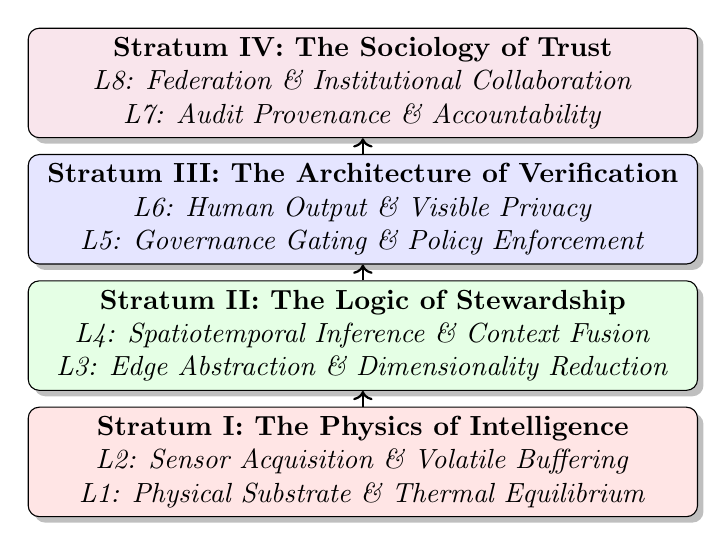
\begin{tikzpicture}[
    node distance=0.2cm,
    layer/.style={rectangle, draw, minimum width=8.5cm, minimum height=1.2cm, align=center, rounded corners, drop shadow, fill=white},
    label/.style={font=\bfseries\small}
]

\node[layer, fill=purple!10] (S4) {
    \textbf{Stratum IV: The Sociology of Trust} \\ 
    \textit{L8: Federation \& Institutional Collaboration} \\
    \textit{L7: Audit Provenance \& Accountability}
};

\node[layer, fill=blue!10, below=of S4] (S3) {
    \textbf{Stratum III: The Architecture of Verification} \\ 
    \textit{L6: Human Output \& Visible Privacy} \\
    \textit{L5: Governance Gating \& Policy Enforcement}
};

\node[layer, fill=green!10, below=of S3] (S2) {
    \textbf{Stratum II: The Logic of Stewardship} \\ 
    \textit{L4: Spatiotemporal Inference \& Context Fusion} \\
    \textit{L3: Edge Abstraction \& Dimensionality Reduction}
};

\node[layer, fill=red!10, below=of S2] (S1) {
    \textbf{Stratum I: The Physics of Intelligence} \\ 
    \textit{L2: Sensor Acquisition \& Volatile Buffering} \\
    \textit{L1: Physical Substrate \& Thermal Equilibrium}
};

\draw[->, thick] (S1) -- (S2);
\draw[->, thick] (S2) -- (S3);
\draw[->, thick] (S3) -- (S4);

\end{tikzpicture}
\caption{The Unified Reference Stack. The system builds upwards from physical constraints (I) to logical reasoning (II), verified trust (III), and social acceptance (IV). The entropic sensitivity of the payload drops at every upward transition.}
\label{fig:stack}
\end{figure}

\subsection{Stratum I: The Physics of Intelligence}
The lowest stratum establishes the physical operating conditions under which the edge node must function. Layer 1 manages Linux kernel parameters, actively maintaining memory volatility and mitigating NAND flash wear through write clustering and compressed RAM-disks. Layer 2 handles high-fidelity sensor acquisition, strictly limiting physical captures to bounded, circular volatile memory buffers.

\subsection{Stratum II: The Logic of Stewardship}
The second stratum performs the critical transformation from raw sensory input to abstract semantic representations. Layer 3 serves as the primary irreversible boundary. High-entropy matrices (such as raw images or audio) are destructively compressed into low-dimensional metadata vectors. Layer 4 then utilizes spatiotemporal logic engines to evaluate behavior and detect actionable events while remaining completely blind to raw identity. 

\subsection{Stratum III: The Architecture of Verification}
Above the reasoning layer sits an architectural verification stratum responsible for enforcing institutional policy and demonstrating system compliance. Layer 5 physically separates algorithmic judgment from transmission authority; a dedicated policy engine must clear the data before network egress is permitted. Layer 6 translates these machine boundaries into human-verifiable proofs, driving abstracted visualizations on public monitors to demonstrate visual anonymity to building occupants \cite{b5}. 

\subsection{Stratum IV: The Sociology of Trust}
The uppermost stratum connects the technical system to broader institutional and social accountability structures. Layer 7 secures tamper-evident, append-only logs of governance decisions to ensure administrative accountability over time. Layer 8 manages federation protocols, leveraging differential privacy and secure aggregation to update neural network weights across distinct campuses without ever pooling centralized raw data \cite{b6}. 

\section{Core Architectural Constraints}

To ensure architectural integrity, the system enforces several non-negotiable operational constraints. If any constraint is violated at runtime, the node immediately transitions into a fail-safe halt state.

\begin{enumerate}
    \item \textbf{Raw Data Non-Persistence:} Raw sensor data must never survive the volatile RAM boundary. The operating system is explicitly hardened to block state persistence to physical disk or swap partitions \cite{b7}.
    \item \textbf{Bounded Temporal Exposure:} Any memory buffer containing raw data is explicitly zeroed within a strict, sub-second timeframe. An independent runtime supervisor enforces this deadline; the specific enforcement mechanism and empirical validation are addressed in companion work on runtime verification.
    \item \textbf{Governance Gating:} The inference engine has zero direct network access. Abstract metadata can only reach the egress module after passing explicit institutional policy checks.
    \item \textbf{Fail-Safe Degradation:} Any operational failure instantly transitions the edge node into a HALT or secure reboot state. The system is structurally prohibited from degrading into an OPEN or permissive bypass state; privacy preservation strictly overrides service availability.
    \item \textbf{Differential Update Restriction:} To stop model inversion attacks, cross-campus model weight updates are barred from containing raw gradient data that could reconstruct local training samples. All federated payloads are subjected to noise injection \cite{b8}.
    \item \textbf{Consent-Gated Processing:} The system generates persistent behavioral embeddings only when user consent is dynamically verified at runtime. If the consent verification service is temporarily unreachable, the architecture defaults to a privacy-safe suspension of embedding generation rather than proceeding without verified authorization.
\end{enumerate}

\section{Inter-Stratum Execution Contracts}

Reliable system behavior requires strict contracts governing communication between architectural layers. Conventional cloud architectures frequently pass opaque pointers or unstructured JSON payloads between microservices. This pattern is often disastrous on constrained edge devices. Parsing JSON consumes valuable CPU cycles, and utilizing unstructured pointers can easily precipitate unintended raw data leaks across security domains.

\subsection{Schema-Constrained Semantic Firewalls}
Communication between the acquisition and logic strata is forced across a highly restricted volatile boundary. The reasoning logic evaluates abstracted data without ever assuming physical memory ownership of the raw data space.

Layer isolation is enforced using Schema-Constrained Semantic Firewalls. In this context, a schema is not merely a serialization format; it acts as a rigid, type-level privacy firewall. If a schema $\mathcal{S}$ lacks explicitly defined fields for raw media, no raw data can mathematically transit the boundary. 

Listing 1 illustrates the canonical protobuf schema bridging this boundary. By design, the schema lacks any fields capable of holding pixel byte arrays or string-based personal identifiers. 

\begin{figure}[htbp]
\textbf{Listing 1: Canonical Protobuf Schema}
\begin{lstlisting}[language=C++]
syntax = "proto3";
package edgeai.core;

// Payload permitted across the volatile boundary
message AbstractEvent {
  uint64 timestamp_ms = 1;
  uint32 spatial_zone_id = 2;
  
  enum EventType {
    UNKNOWN = 0;
    HAND_RAISE = 1;
    GAIT_ANOMALY = 2;
    ACOUSTIC_IMPULSE = 3;
  }
  EventType type = 3;
  
  // Ephemeral tracing token (Valid for 1 frame only)
  uint64 session_ephemeral_token = 4;
  
  // Dimensionality bounded constraint vector
  repeated float geometric_keypoints = 5; 
}
\end{lstlisting}
\caption{The formal payload schema. The execution contract physically prevents raw image or audio fields from passing to the Inference layer, supporting abstraction constraints at the rigid type-definition level.}
\label{fig:protobuf}
\end{figure}

Schema evolution requires precise version pinning across the edge node fleet to prevent decoding mismatches during staggered institutional updates.

\subsection{The Temporal Budget Contract}
Beyond schema-level isolation, the architecture imposes a globally verifiable temporal contract on the execution pipeline. The entire runtime sequence---spanning sensor capture, abstraction, logic evaluation, and final buffer destruction---must complete within a hard temporal budget. An independent supervisor monitors pipeline progress against this deadline. Should the execution engine fail to meet its temporal contract, the system deterministically transitions to a privacy-safe halt state, ensuring that deadline violations degrade into secure shutdowns rather than unauthorized data retention.

\section{The Life of an Event: End-to-End Sequence}

The interaction between architectural layers can be illustrated by tracing the lifecycle of a single spatiotemporal event. (Figure \ref{fig:sequence}).

\begin{figure}[htbp]
\centering
\resizebox{\columnwidth}{!}{
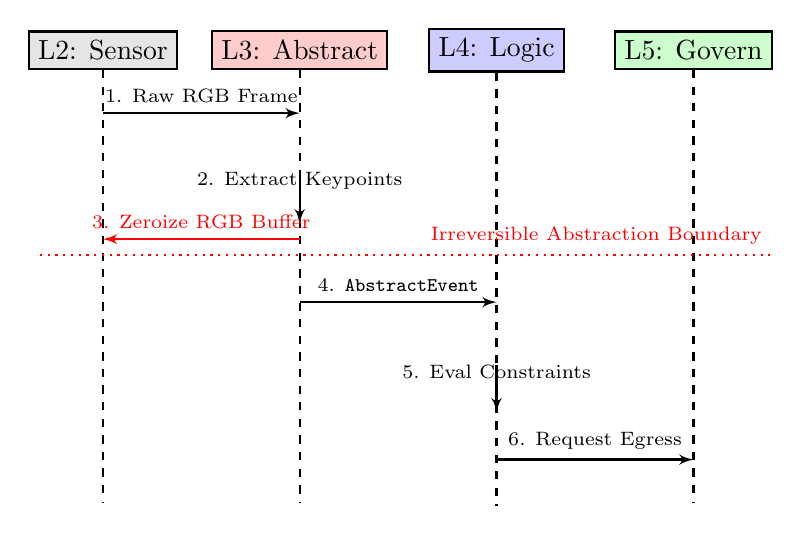
\begin{tikzpicture}[>=latex']
    \node (L2) at (0,0) [rectangle, draw, thick, minimum width=1.5cm, fill=gray!20] {L2: Sensor};
    \node (L3) at (2.5,0) [rectangle, draw, thick, minimum width=1.5cm, fill=red!20] {L3: Abstract};
    \node (L4) at (5,0) [rectangle, draw, thick, minimum width=1.5cm, fill=blue!20] {L4: Logic};
    \node (L5) at (7.5,0) [rectangle, draw, thick, minimum width=1.5cm, fill=green!20] {L5: Govern};

    \draw [thick, dashed] (L2.south) -- +(0,-5.5);
    \draw [thick, dashed] (L3.south) -- +(0,-5.5);
    \draw [thick, dashed] (L4.south) -- +(0,-5.5);
    \draw [thick, dashed] (L5.south) -- +(0,-5.5);

    \draw [->, thick] (0,-0.8) -- node[above, font=\scriptsize] {1. Raw RGB Frame} (2.5,-0.8);
    \draw [->, thick] (2.5,-1.6) -- node[above, font=\scriptsize] {2. Extract Keypoints} (2.5,-2.2);
    \draw [->, thick, red] (2.5,-2.4) -- node[above, font=\scriptsize] {3. Zeroize RGB Buffer} (0,-2.4);
    
    \draw [->, thick] (2.5,-3.2) -- node[above, font=\scriptsize] {4. \texttt{AbstractEvent}} (5,-3.2);
    \draw [->, thick] (5,-4.0) -- node[above, font=\scriptsize] {5. Eval Constraints} (5,-4.6);
    \draw [->, thick] (5,-5.2) -- node[above, font=\scriptsize] {6. Request Egress} (7.5,-5.2);

    \draw [red, thick, dotted] (-0.8, -2.6) -- (8.5, -2.6) node[above left, font=\scriptsize, text=red] {Irreversible Abstraction Boundary};
\end{tikzpicture}
}
\caption{End-to-End Event Sequence. The critical action occurs at Step 3: the raw data capture is explicitly destroyed \textit{before} the abstracted protobuf payload is transmitted to the Logic Layer (Step 4).}
\label{fig:sequence}
\end{figure}

\begin{enumerate}
    \item \textbf{Ingestion:} A frame lands in a bounded volatile buffer utilizing a zero-copy pipeline, prompting the supervisor to immediately start the destruction countdown clock.
    \item \textbf{Abstraction:} A lightweight neural network extracts geometric keypoints from the frame. Crucially, the original RGB frame is subsequently overwritten and explicitly destroyed, proactively preventing the OS from caching it in the background.
    \item \textbf{Reasoning:} The continuous stream processing engine takes the abstract event protobuf and evaluates local spatiotemporal heuristics.
    \item \textbf{Governance:} Upon generating a metadata payload for a positive match, the Governance Filter queries active institutional policy to verify whether logging the event is currently permitted.
    \item \textbf{Audit:} If cleared by policy, the governance decision is tamper-evidently recorded in a local append-only log, securing the record against insider tampering.
\end{enumerate}

\section{Physical Deployment Topologies}

A theoretical reference architecture offers limited value if it cannot map reliably onto physical hardware. We evaluate the logical stack against three distinct deployment profiles to verify physical viability.

\subsection{Profile A: The Autonomous Micro-Edge}
This profile represents bandwidth-starved environments characterized by highly intermittent network reliability.
\begin{itemize}
    \item \textbf{Hardware:} A commodity ARM-based System-on-Chip (SoC) mounted directly inside the room. Under sustained inference loads with passive cooling, thermal throttling is expected within typical edge thermal envelopes. The architecture accommodates this through dynamic, policy-driven frame-rate reduction that maintains compliance with CFAS constraints even under degraded thermal conditions.
    \item \textbf{Layer Mapping:} Operations L1 through L7 run entirely on the physical node. 
    \item \textbf{Network Dependency:} Minimal. The system remains autonomous, synchronizing metadata via MQTT Store-and-Forward protocols only when network uplinks are restored.
\end{itemize}

\subsection{Profile B: The Campus Macro-Edge Cluster}
This configuration represents modern university environments equipped with high-speed fiber LAN infrastructure.
\begin{itemize}
    \item \textbf{Hardware:} Lightweight IP cameras blasting RTSP streams to a localized server rack down the hall.
    \item \textbf{Layer Mapping:} Sensors just capture video. The abstraction, logic, and governance layers execute on the high-throughput local cluster. 
    \item \textbf{Security Boundary:} The internal video stream is isolated on a completely non-routable VLAN. The local server cluster serves as the absolute destruction boundary.
\end{itemize}

\subsection{Profile C: Hybrid Fog Consortium}
This represents multi-campus consortiums attempting to train generalized behavioral models without centralizing their underlying student datasets \cite{b9}.
\begin{itemize}
    \item \textbf{Layer Mapping:} Individual campuses run Profile B. The L8 Federation layer wakes up, allowing the distinct campuses to securely swap model weight updates (gradients) using decentralized optimization \cite{b10}. The exact federated optimization algorithm is flexible, provided it operates strictly within the boundary constraints.
\end{itemize}

\section{Trade-off Space Analysis}

Architectures built around strict privacy constraints inevitably sacrifice a degree of performance and analytical flexibility. This reference model forces four primary trade-offs.

\subsection{Latency vs. Privacy Boundaries}
The strict requirement to wipe raw buffers within a predefined Time-To-Live (TTL) naturally places an absolute ceiling on inference latency. Letting $\tau_p$ represent the privacy TTL and $\tau_i$ represent the model's inference latency, the unyielding constraint becomes $\tau_i \le \tau_p$. 
The feasible model class is formally defined as:
\begin{equation}
\mathcal{M} = \{m \mid \text{latency}(m) \le \tau_p\}
\end{equation}
\textit{Architectural Consequence:} Consequently, massive, highly accurate foundation models often fall entirely outside the feasible class under strict temporal constraints and simply cannot be deployed.

\subsection{Utility vs. Abstraction}
Because the architecture explicitly destroys raw frames at L3, the system permanently abandons the ability to perform retrospective analytics on unforeseen phenomena. Should administrators later decide to track a novel physical attribute, they cannot query historical footage; only the predefined structural keypoints are preserved.
\textit{Architectural Consequence:} Extreme limits on retrospective flexibility. Semantic classes must be perfectly defined prior to deployment execution.

\subsection{Bandwidth vs. Centralized Telemetry}
Operating within a federated topology requires exchanging millions of model parameters between edge nodes and aggregation servers, rather than simply streaming raw images to a cloud repository.
\textit{Architectural Consequence:} While federated learning absolutely reduces raw-data exposure, the periodic burst transmissions of heavy gradient updates place a distinctly different, highly bursty strain on institutional network infrastructure.

\subsection{Auditability vs. Minimal Data Retention}
To maintain the tamper-evident log (L7), the system must persistently store metadata regarding its own governance decisions to ensure administrative accountability.
\textit{Architectural Consequence:} However, saving audit logs inherently requires persisting metadata. This slightly widens the systemic attack surface for bad actors attempting deductive correlation attacks. Balancing detailed, verifiable auditability against the foundational principle of data minimization remains a persistently difficult architectural tightrope.

\section{Related Work}

The design of reference architectures for intelligent environments has been addressed at multiple abstraction levels. The NIST Fog Computing Conceptual Model \cite{b26} and ISO/IEC 30141 IoT Reference Architecture \cite{b27} provide broad structural frameworks but do not enforce privacy constraints at the architectural level. Edge computing surveys \cite{b11, b22} catalogue deployment patterns but typically treat privacy as an orthogonal concern rather than a first-class architectural constraint.

Within privacy-preserving systems, Cavoukian's Privacy-by-Design principles \cite{b7} establish high-level design guidance but do not prescribe specific architectural enforcement mechanisms. Denning's lattice model of information flow \cite{b25} provides a formal basis for multilevel security, and the present architecture's irreversible abstraction boundary can be interpreted as a strict downward information flow constraint within that framework. More recent work on confidential computing \cite{b4} addresses hardware-level memory isolation but assumes trusted execution environments not available on commodity edge hardware.

In the smart campus domain specifically, existing systems such as those surveyed by Shi et al. \cite{b11} and Mao et al. \cite{b22} focus on computational offloading and latency optimization. These architectures generally lack the integrated governance gating, adversary-tiered defense mapping, and schema-enforced irreversibility boundaries that CFAS provides.

The adversary modeling approach adopted here draws on the formal adversary capability algebra established in companion work \cite{b20_threat}, which provides the mathematical tuple definitions and bounding assumptions. The present paper contributes the architectural defense mapping---associating each adversary tier with the specific stratum that neutralizes its capabilities---rather than the formal adversary definitions themselves.

\section{Conclusion}

This paper presented a unified architectural framework for privacy-oriented edge intelligence. Rather than addressing hardware constraints, inference pipelines, governance mechanisms, and sociotechnical transparency as independent research topics, the architecture organizes them into a single layered framework guided by Constraint-First Architectural Synthesis. 

The analysis shows that physical limitations, irreversible abstraction boundaries, strict governance gating, and accountability logging can coexist within a coherent deployment stack. Although several trade-offs remain unavoidable---particularly those involving latency limits, model flexibility, and audit granularity---the framework provides a structured approach for navigating those constraints. 

Ultimately, responsible deployment of intelligent environments cannot depend on policy statements alone. It requires architectural decisions that embed privacy and governance constraints directly into the operational structure of the system.

\begin{thebibliography}{00}

\bibitem{b1} H. Nissenbaum, \textit{Privacy in Context: Technology, Policy, and the Integrity of Social Life}, Stanford University Press, 2009.
\bibitem{b2} European Union, ``General Data Protection Regulation (GDPR),'' \textit{Official Journal of the European Union}, 2016.
\bibitem{b3} J. H. Saltzer and M. D. Schroeder, ``The protection of information in computer systems,'' \textit{Proceedings of the IEEE}, vol. 63, no. 9, pp. 1278-1308, 1975.
\bibitem{b4} J. A. Halderman et al., ``Lest we remember: cold boot attacks on encryption keys,'' in \textit{USENIX Security Symposium}, 2008.
\bibitem{b5} M. R. Endsley, ``Toward a theory of situation awareness in dynamic systems,'' \textit{Human Factors}, vol. 37, no. 1, pp. 32-64, 1995.
\bibitem{b6} P. Kairouz et al., ``Advances and Open Problems in Federated Learning,'' \textit{Foundations and Trends in Machine Learning}, vol. 14, no. 1--2, pp. 1-210, 2021.
\bibitem{b7} A. Cavoukian, ``Privacy by Design: The 7 Foundational Principles,'' \textit{Information and Privacy Commissioner of Ontario}, 2009.
\bibitem{b8} C. Dwork and A. Roth, ``The Algorithmic Foundations of Differential Privacy,'' \textit{Foundations and Trends in Theoretical Computer Science}, 2014.
\bibitem{b9} M. Satyanarayanan, ``The Emergence of Edge Computing,'' \textit{Computer}, vol. 50, no. 1, pp. 30-39, 2017.
\bibitem{b10} B. McMahan et al., ``Communication-Efficient Learning of Deep Networks from Decentralized Data,'' in \textit{Proc. AISTATS}, 2017.
\bibitem{b11} W. Shi et al., ``Edge Computing: Vision and Challenges,'' \textit{IEEE Internet of Things Journal}, vol. 3, no. 5, pp. 637-646, 2016.
\bibitem{b12} J. D. Lee and K. A. See, ``Trust in automation: Designing for appropriate reliance,'' \textit{Human Factors}, vol. 46, no. 1, pp. 50-80, 2004.
\bibitem{b13} J. Arlat et al., ``Fault injection for dependability validation: A methodology and some applications,'' \textit{IEEE Transactions on Software Engineering}, 1990.
\bibitem{b14} M. Leucker and C. Schallhart, ``A brief account of runtime verification,'' \textit{Journal of Logic and Algebraic Programming}, 2009.
\bibitem{b15} N. G. Leveson, \textit{Safeware: System Safety and Computers}, Addison-Wesley, 1995.
\bibitem{b16} S. Zuboff, \textit{The Age of Surveillance Capitalism}, PublicAffairs, 2019.
\bibitem{b17} L. Sweeney, ``k-anonymity: A model for protecting privacy,'' \textit{International Journal of Uncertainty, Fuzziness and Knowledge-Based Systems}, 2002.
\bibitem{b19} J. Kim et al., ``A Survey on Flash Translation Layer,'' \textit{IEEE Transactions on Consumer Electronics}, 2010.
\bibitem{b20} P. Desnoyers, ``Analytic Modeling of SSD Write Performance,'' \textit{SYSTOR}, 2012.
\bibitem{b21} R. Natella et al., ``Assessing dependability with software fault injection: A survey,'' \textit{ACM Computing Surveys}, 2016.
\bibitem{b22} Y. Mao et al., ``A survey on mobile edge computing,'' \textit{IEEE Communications Surveys \& Tutorials}, 2017.
\bibitem{b23} F. Pasquale, \textit{The Black Box Society}, Harvard Univ. Press, 2015.
\bibitem{b24} T. Li et al., ``Federated learning: Challenges, methods, and future directions,'' \textit{IEEE Signal Processing Magazine}, 2020.
\bibitem{b25} D. E. Denning, ``A lattice model of secure information flow,'' \textit{Communications of the ACM}, 1976.
\bibitem{b26} NIST, ``Fog Computing Conceptual Model,'' \textit{NIST Special Publication 500-325}, 2018.
\bibitem{b27} ISO/IEC, ``Internet of Things (IoT) --- Reference Architecture,'' \textit{ISO/IEC 30141:2018}, 2018.

\bibitem{b20_threat} S. S. Kumar, ``Formal Threat Model and Trusted Computing Base Definition for Architecturally Irreversible Edge AI,'' in \textit{Proc. IEEE Security \& Privacy Workshops}, 2026.

\end{thebibliography}

\end{document}
